%---Document Class---%
\documentclass[12pt]{report}

%---Packages---%
\usepackage[utf8]{inputenc} %Danish letters
\usepackage{authblk} %Title
\usepackage{graphicx}
\usepackage{sectsty}
\usepackage{caption}
\usepackage{subcaption}
\usepackage{listings}
\usepackage[hidelinks]{hyperref} %Emails in Title

\usepackage[usenames,dvipsnames]{xcolor}


%---Colors---%
\definecolor{chapterColor}{HTML}{004685}
\definecolor{sectionColor}{HTML}{087D9C}
\definecolor{subSectionColor}{HTML}{07928A}
\definecolor{defaultColor}{HTML}{222222}

\chapterfont{\color{chapterColor}}
\sectionfont{\color{sectionColor}}
\subsectionfont{\color{subSectionColor}}
\color{defaultColor}

%---Fonts---%
\renewcommand\textbullet{\ensuremath{\bullet}}
\usepackage[default]{raleway}
\usepackage[T1]{fontenc}

%---Page Setup---%
\usepackage[a4paper, margin=3cm]{geometry}
\setlength{\parindent}{0em}
\setlength{\parskip}{1em}

\lstdefinestyle{customc}{
    belowcaptionskip=1\baselineskip,
    breaklines=true,
    xleftmargin=\parindent,
    language=C,
    showstringspaces=false,
    basicstyle=\footnotesize\ttfamily,
    keywordstyle=\bfseries\color{green!40!NavyBlue},
    commentstyle=\itshape\color{purple!40!NavyBlue},
    identifierstyle=\color{black},
    stringstyle=\color{orange},
    tabsize=4,
    numbers=left,
    numberstyle=\tiny\color{gray},
}

\lstset{style=customc}

%--- Bibliography ---%
\usepackage[backend=bibtex,bibencoding=ascii]{biblatex}
\addbibresource{chapters/cha_bibliography/bibliography.bib}


%---Begin Document---%
\newcommand{\documentTitle}{Design, simulation and development of a bipedal locomotion platform  for human-like gaits studies}
\newcommand{\documentType}{Master Thesis}

\newcommand{\institute}{University of Southern Denmark}
\newcommand{\department}{Faculty of Engineering}
\newcommand{\program}{MSc in Engineering, Robot Systems}
\newcommand{\course}{Robot System Design}

\newcommand{\authorOne}{Jorge Rodriguez Marin}
\newcommand{\authorTwo}{Ignacio Torroba Balmori}

%---Begin Document---%
\begin{document}
    \pagenumbering{gobble} % Remove warnings of number page
	%!TEX root = ../../report.tex

% Title Page
\begin{titlepage}
	\begin{center}
	
\includegraphics[width=60mm,keepaspectratio]{figures/sdu_logo}\\
	\vspace{0.3cm}
	\textbf{\institute}\\
	\textmd{\department}\\
	\textmd{\program} - \textmd{\course}\\[4cm]

	\vspace{0.4cm}
	{\huge \bfseries \documentTitle}
	\\
	\vspace{0.5cm}
	{\large \documentType}
	\\[2cm]

	\begin{tabular}{c}
	 \makebox[4cm]{\emph{Authors}} \\
	 \makebox[4cm]{\authorOne} \\
	 \makebox[4cm]{\authorTwo} \\
	\end{tabular}

	\vfill
	{\large \today}
	\end{center}
\end{titlepage}

    \pagenumbering{arabic} % Remove warnings of number page
    \setcounter{page}{2}

    \tableofcontents\thispagestyle{empty}\vfill % No number page
	%\tableofcontents

	%!TEX root = ../report.tex
\chapter{Introduction}
\label{chap:introduction}

\section{Overall description}
The goal of this project is 

\subsection{Report structure}
The report is organized so it starts with	
    %!TEX root = ../../report.tex
\chapter{Mechanical Design} % (fold)
\label{cha:mechanical_design}
In here bla bla bla

%!TEX root = ../../../report.tex
\section{Limb structure} % (fold)
\label{sec:limb_structure}



% section limb_structure (end)


% chapter mechanical_design (end)

    %!TEX root = ../../report.tex
\chapter{Discussion} % (fold)
\label{cha:discussion}

%Alternatives to the use of the main board's input pins

% chapter discussion (end)
    %!TEX root = ../../report.tex
\chapter{Conclusions and further work} % (fold)
\label{cha:conclusions}
As a general conclusion, the creation of a coherent simulation environment and the construction of a robust, low-cost and reconfigurable bipedal locomotion platform has been achieved.
The ultimate goal was to contribute on the on-going line of research in locomotion control at the AI department at the Maersk Mc-Kinney Møller Institute, and RuBi offers a good compromise between features and affordability.
From the bringing up of the robot to the set up of the simulation environment,  including easy manufacturability and maintenance or code examples, RuBi is focused on facilitating the development of new locomotion controllers for teaching or research.
The platform aims to create a bridge between the creation of controllers and their testing, which ultimately will speed up the development workflow and the possible experiments to be carried out in the area by the Embodied AI \& Neurorobotics Lab.

However, much work was also planned to be left for further improvements of the RuBi study framework since, as said before, from the beginning this project was meant to be continued.
This reason has led to the creation of the detailed and comprehensive documentation contained in this report, its appendixes, the assembly manuals \footnote{https://www.youtube.com/watch?v=rceASqIJ4HQ} and the online repository \cite{rubi_repo}.
Their aim is to provide the tools to easily and quickly understand and master the use of RuBi.
From here, the uses of the platform are left to the imagination of future users.

\section{Further work} % (fold)
\label{sec:further_work}
The missing work that laid on the original scope of this thesis but could not be conducted is mentioned here for each of the main areas of the project.
Besides, some enhancements and experimental setups already suggested are summarized below.

%%% Mechanics
% Analyze all the mechanical stresses of individual parts and an assembly analysis
% Improve fastening for motor interfaces
% Improve foot shape in order to help the step
% Reinforce fragile sections in 3D printed parts
% Develop a method to tension the belts
% Re-implement parallel spring holder to make it easier
% Add more features to the structure
% Implement a jumping platform
From the robot mechanics perspective, the very basic tests conducted seem to yield the need of reinforcing the hip structure, keeping its original design but widening its size.
Also the robot holder on the external structure needs to be 3D-printed again to adjust its clearances due to the use of a different 3D printer for its creation, because of its size.
The fastening of the motor interfaces could also be improved as it has shown to be a valid design but with some leaks when clamping.
Other future improvements could be the development of a more accurate method to measure the tension of the belts or a redesign of the parallel spring holder to make faster the change of the torsion spring.
Besides, in \ref{cha:experiments} it was suggested the construction of a small platform with additional contact sensors for experiments in vertical jumps.
This could be necessary since the current contact sensors are placed on the heels, but the first landing point when hopping is the toes.
Since a solution to the placement of more sensors on the current foot design could not be found, it is proposed to install off-board sensors to supply that information.

%%% Mathematical model
% Development of a ground-contact force model --> the current one is a Normal function
The calculations carried out to model the robot and its application have been created in MATLAB and used to evaluate the needs on hardware for RuBi.
The models are left in an early development stage since they were meant to rely on experimental data to assess its accuracy and enhance them.
However, with a fully operative prototype of the robot, the dynamic model can be further tested and used to detect and carry out improvement on the robot dynamics for a better performance, as it has been used for during its design. 
The construction of the dynamic model of a robot must be led by the seek of a balanced trade-off between accuracy in the representation of the actual device and simplicity to handle and understand its behavior.
This stage has been tried to be found here through the use of the assumptions about the real world and the robot capabilities.
A first suggestion for further improvement of the model would be to minimize these assumptions and try to model every dynamic term and scenario.
However, as explained, this does not necessarily yield a better output of the process.
Therefore it is left as further work the adaption of the mathematical model as required by the user in the need of a more advanced solution, since assessing the quality of a model is not a trivial task and depends on its use.

%%% Electronics
% Alternatives to the use of the main board's input pins
% Implement a method to read easily from I/O
% Add more sensors to the robot: IMU
% Add absolute encoders or improve the initialization
% Reduce the network latency by using 5Ghz or by using Ethernet
% Study the general latency of the system and how it affect to the measurements
% Develop a easier and safer system for powering the robot
The electronic implementation of RuBi has proved to be robust and valid, but the set of possibilities that offers has not been fully exploited.
The ROS Control interface has to be extended to include position control and readings from new sensors besides the angular encoders in the motors.
The feet contact sensors have been installed but not plugged to the processor due to lack of documentation on the main board.
This could be easily fixed adding some external circuitry as an Arduino, for instance, or exploring the capabilities of the existing I/O pins on the motor controller boards.
Furthermore, abilitating new GPIOS on the hardware system could allow for more and more complex on-board sensors as an IMU or light sensors to improve self-awareness.
Currently the relative encoders on the motors are manually initialized by placing the joints on their mechanical maximum extension.
This should be enhanced to create an automatic solution.

%%% Simulation
% Add springs to the simulation
% Improve the simulation by modifying physic parameters until reach reality-like results
% Add color and textures to the simulation
% Implement more experiments within the simulation
Ultimately, the simulation model of RuBi was designed with direct drive transmission in the joints.
The addition of springs to the model could lead to more realistic results, though this has to be tested.
The adjustment of certain simulation values as the time step or some in the model of the robot, as the dynamic rotational friction, have to be done based on results taken from the real robot.
The model can also be improved by attaching more realistic visual characteristics like adding colors and textures to the parts.
The possibilities of Gazebo have not been squeezed so the inclusion of new simulation environments, sensors or other models is left to further research.

% section further_work (end)

% chapter conclusions (end)
    %!TEX root = ../../report.tex

\chapter{Simulation} % (fold)
\label{cha:simulation}
This chapter is meant to answer the questions what, why and how a simulator takes part in the framework.
Starts with a motivation section \ref{sec:sim_motivation} which defines the scope of the simulator
 in the project, followed by a comparison of simulators \ref{sec:sim_comparison_of_simulators} and how to define a robot and its environment in it \ref{sec:robot_definition}; in the next section \ref{sec:robot_creation} is explained how the simulation model of the legs has been created and how to add new features, whilst the creation of the environment is dealt in the section \ref{sec:environment_creation}; finishes with a how-to dedicated section for launching the simulation from scratch in \ref{sec:how_to_simulate}.
%!TEX root = ../../../report.tex
\section{Motivation} % (fold)
\label{sec:sim_motivation}
In the previous chapters the design of a human-proportional biped has been presented. 
The robot has been developed with security systems in both, software and hardware, that prolong the operating life of the robot. 
Nevertheless, every device in real life is prone to suffer damage which translates in to money and time for the user.
By forming part of the toolbox offered in the framework, a comprehensive biped simulation is given so the user can both work with the same algorithms in real and simulated life.

Whilst not being a complete replacement of the real life, it offers a similar experience what allows to do qualitative research.
As an example, neuronal networks or reinforcement learning algorithms, that learn by experience, can be developed faster in the simulator and then transfered to the real robot, reducing the workflow and the need of resources of the user and justifying its use.

A simulator consists basically of two elements: a physical engine and a graphical engine.
Whilst the first one is in charge of calculate all the physical interactions that the agent suffers, the second one offers the visual experience.
A congruent simulator with the presented framework will satisfy two conditions:
\begin{enumerate}
  \item The effort for testing among the simulation and real life must be minimized
  \item The results must be as closer to real life as possible. This includes multiphysics support (mechanical contacts, different aspects of tribology, wind, water...) but within a fair trade-off with computational speed.
\end{enumerate}

% section motivation (end)
%!TEX root = ../../../report.tex
\section{Comparison of simulators} % (fold)
\label{sec:sim_comparison_of_simulators}
When choosing a simulation platform there are several factors to have into account.
Three robotic simulators have been analyzed and compared. 
These are: LPZ Robots \cite{lpzrobots} (Figure \ref{fig:lpzrobots_example}), V-Rep \cite{vrep} (Figure \ref{fig:vrep_example}) and Gazebo \cite{gazebo} (Figure \ref{fig:gazebo_example}).
Some comparisons can be found in the literature as \cite{nogueiracomparative} or \cite{staranowicz2011survey} however the predominant criteria has been their integration with ROS.

\begin{figure}[hb!]
  \begin{subfigure}{.33\textwidth}
    \centering
    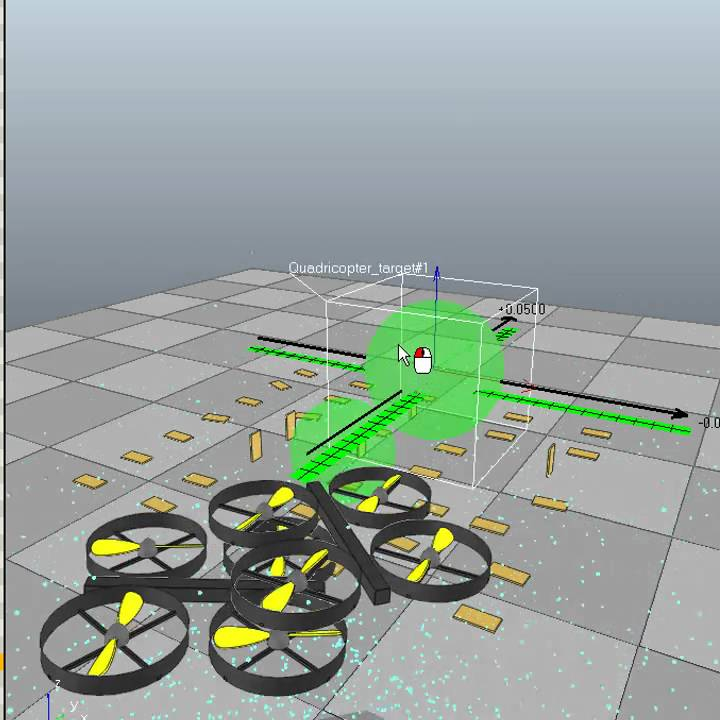
\includegraphics[width=.95\linewidth]{figures/vrep_example}
    \caption{V-Rep}
    \label{fig:vrep_example}
  \end{subfigure}%
  \begin{subfigure}{.33\textwidth}
    \centering
    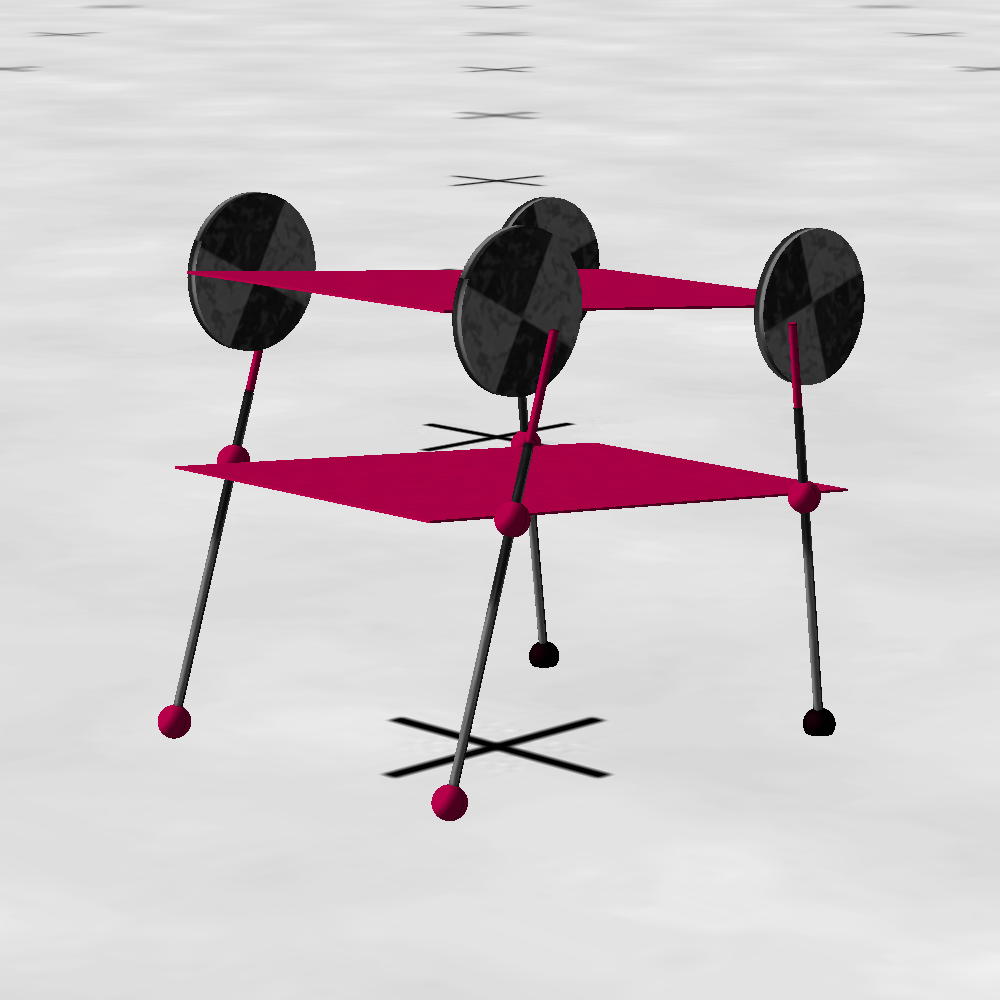
\includegraphics[width=.95\linewidth]{figures/lpzrobots_example}
    \caption{LPZ Robots}
    \label{fig:lpzrobots_example}
  \end{subfigure}
  \begin{subfigure}{.33\textwidth}
    \centering
    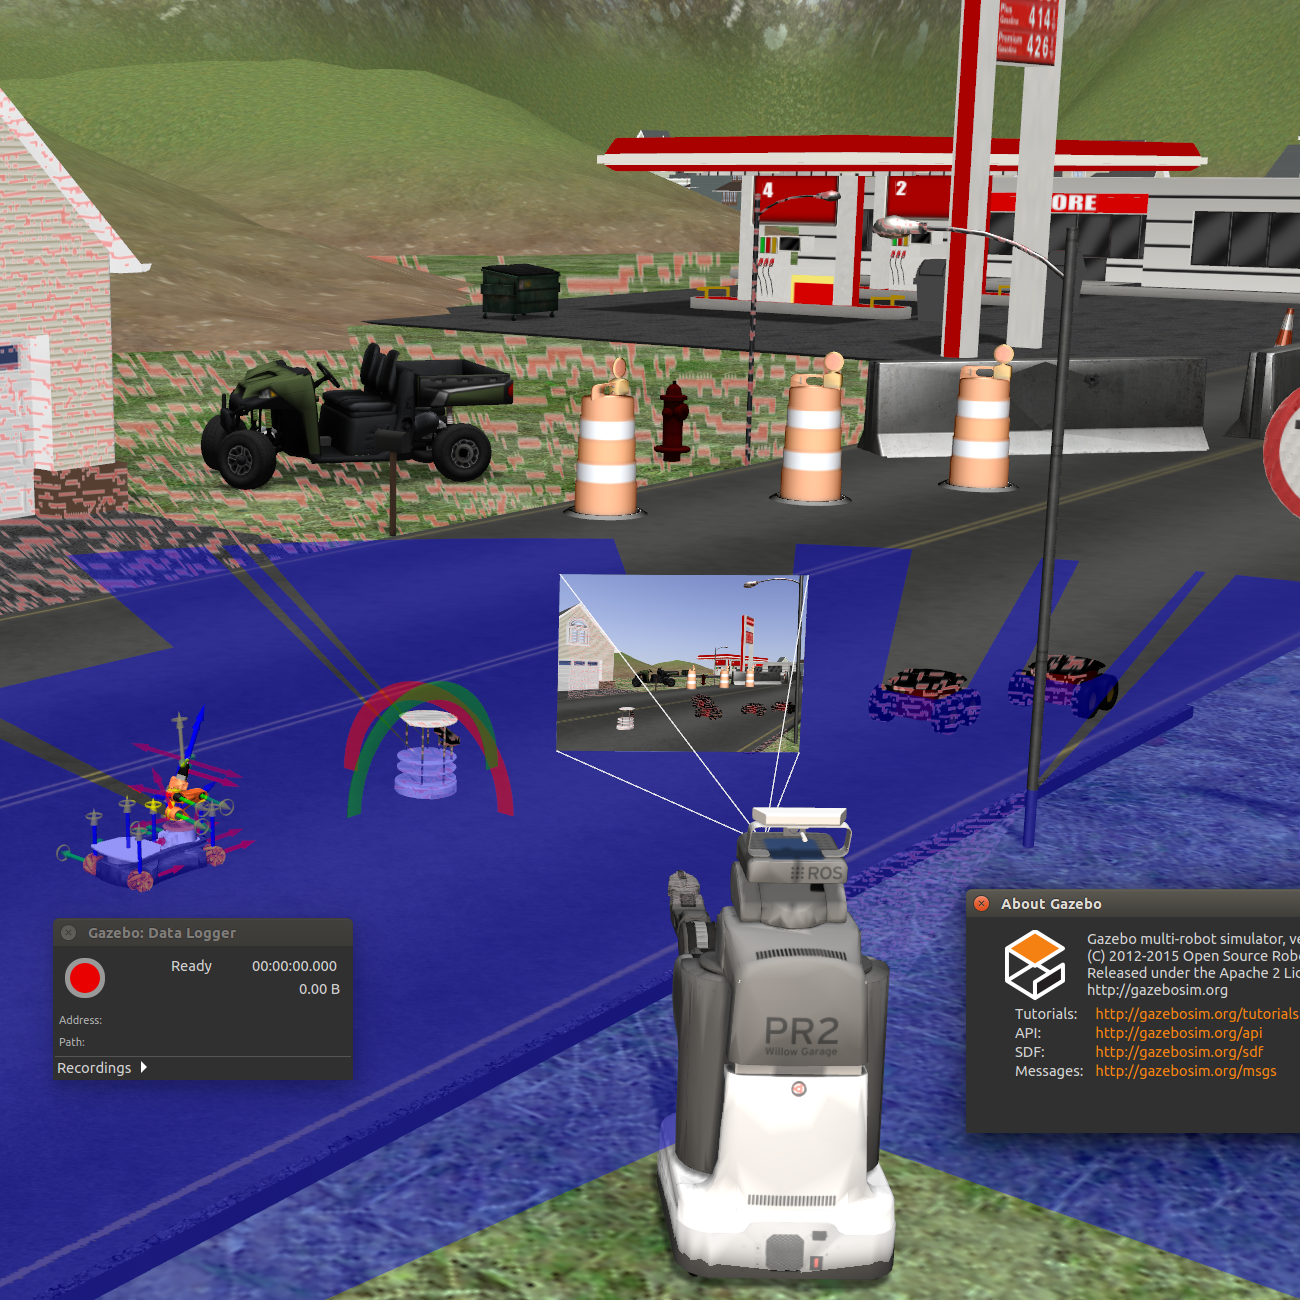
\includegraphics[width=.95\linewidth]{figures/gazebo_example}
    \caption{Gazebo}
    \label{fig:gazebo_example}
  \end{subfigure}
  \caption{Simulation examples of the software analyzed.}
  \label{fig:simulation_comparison}
\end{figure}

The RuBi robot is mainly targeted to be used in the AI department at the Maersk Mc-Kinney Møller Institute, where the toolbox GoRobots is being developed.
This is a set of tools, from a neuronal networks API to a genetic algorithm engine, written in C++ than is meant to be simulator-independent.
However, in order to provide a more general and supported simulation and development environment for the user, ROS Jade \cite{ros} has been selected as the tool to use.
The whole set of instruments provided in ROS along with its easy extendability give the opportunity to use the controllers and tools already developed in GoRobots.
Despite the fact that the three simulators compared have a C++ interface that would allow to interface them with ROS, Gazebo is already fully supported and integrated in ROS, making it the logic choice.
This reduces the learning curve of a new user and the installation process is easier due to it is included in the Open Source Robotics Foundation (OSRF) repositories.

Regarding the second condition, Gazebo has the feature of changing the physics engine in the beginning of the simulation, it has multiphysics support (fluids, electromagnetism...), it allows to load external geometries from STL or Collada and, the most important, has an active community behind it providing support and documentation. These are the reasons for selecting Gazebo as the simulator for the RuBi platform.
In \cite{physics_engine_gazebo_comparison}, a comparison with the different physical engines is carried out.
For the sake of simplicity the default one, Open Dynamics Engine (ODE), has been used, although the others have been tested.

% section comparison_of_simulators (end)\[
%!TEX root = ../../../report.tex
\section{Robot definition} % (fold)
\label{sec:robot_definition}
As in May of 2016, ROS Jade ecosystem has different formats to describe a robot.
These are SDF, URDF and Xacro.
At some point they are all transformed to a unique sort of format but the decision of how to express the robot for the simulation is needed from the beginning.


\begin{enumerate}
  \item \textbf{URDF \footnote{http://wiki.ros.org/urdf}}: is an open standard used in all the simulators mentioned or others like RobWork \cite{robwork}. 
  It allows to define all the properties of a single robot but lacks other which are important when simulating. 
  It is mainly used for visual representations or schematic robot definitions.
  \item \textbf{Xacro \footnote{http://wiki.ros.org/xacro}}: is a parametric format that easy the writing of the URDF.
  It allows logic conditions like \textit{if, for} and from ROS Jade any virtual python condition.
  This code is then compiled into a URDF automatically which give Xacro complete interoperability with URDF readers.
  \item \textbf{SDF \footnote{http://sdformat.org}}: adapted to the current requirements of the simulation environments.
  With it can be defined from \textit{worlds} to air properties in the case or UAV simulations.
\end{enumerate}

Despite SDF contains more information, there are several tools in ROS Jade that make use of URDF.
Two of them are RViz and ROS Control, explained in the section \ref{sub:ros_control}.
As this last one is a pillar of the framework itself, the decision of making use of URDF as format for describing the robot was taken.
However, the robots developed have been written in Xacro due to the tools that easy the coding of the robot.
% section robot_definition (end)
%!TEX root = ../../../report.tex
\section{Robot creation} % (fold)
\label{sec:robot_creation}
One of the goals of the framework is to easy its continuity, thus this section is dedicated to explain how the robot was created.

A robot is defined as a set of links jointed.
A link contains at least three blocks of information:
\begin{enumerate}
   \item The collision model: used to calculate the collisions with other agents in the simulation.
   \item The visual model: uniquely used for visual purposes.
   \item The inertial information: defines physical properties like the mass and the moments of inertia of the link.
\end{enumerate} 

A trade-off must be found for the precision of the collision model between accuracy and speed.
The more detailed is the model, the higher will be computation time which translates into more accuracy and more computation time.
The general advice is to have two simulation models: one for visual purposes and the other one for collisions.

In the case of the links of presented robot, the visual models are obtained directly by exporting the parts from SolidWorks whilst the collision models are made of primitive gazebo shapes (cubes, cylinders, spheres...) for the whole body but the feet.
Due to the robot is not meant to hit anything, the possible collisions in the body are not a priority, then each link is represented as a cylinder of the same length of the CAD model and of a radius enough to cover the whole part.
An example can be seen in the figure \ref{fig:collision_model}.

The moments of inertia of each individual link are obtained directly from SolidWorks.
The CAD model includes the materials and thus the masses.
From these, the program is able to calculate the moments of inertia.
The figure \ref{fig:moments_of_inertia} shows the representation of these in the simulation.


\begin{figure}[hb!]
  \centering
  \begin{subfigure}{.45\textwidth}
    \centering
    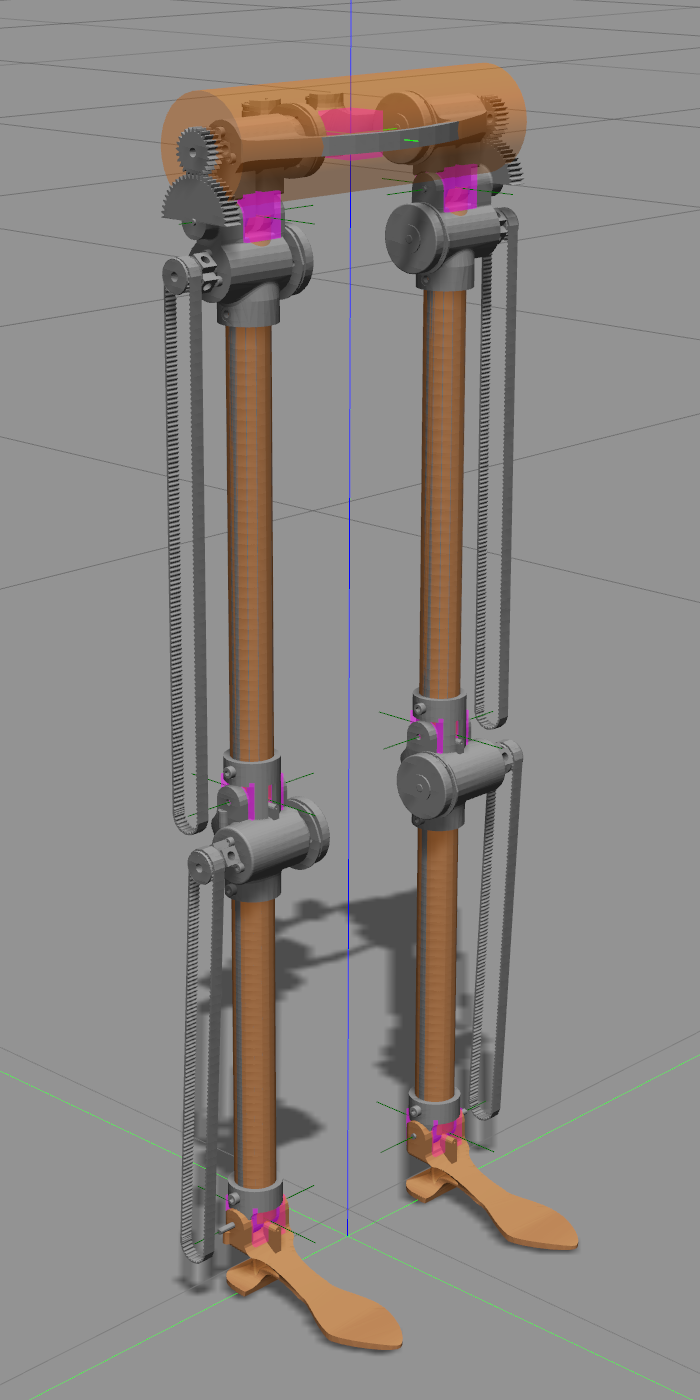
\includegraphics[width=.5\linewidth]{figures/gazebo_collision_model.png}
    \caption{Gazebo showing the visual model, the moments of inertia and the collision model}
    \label{fig:collision_model}
  \end{subfigure}
  \begin{subfigure}{.45\textwidth}
    \centering
    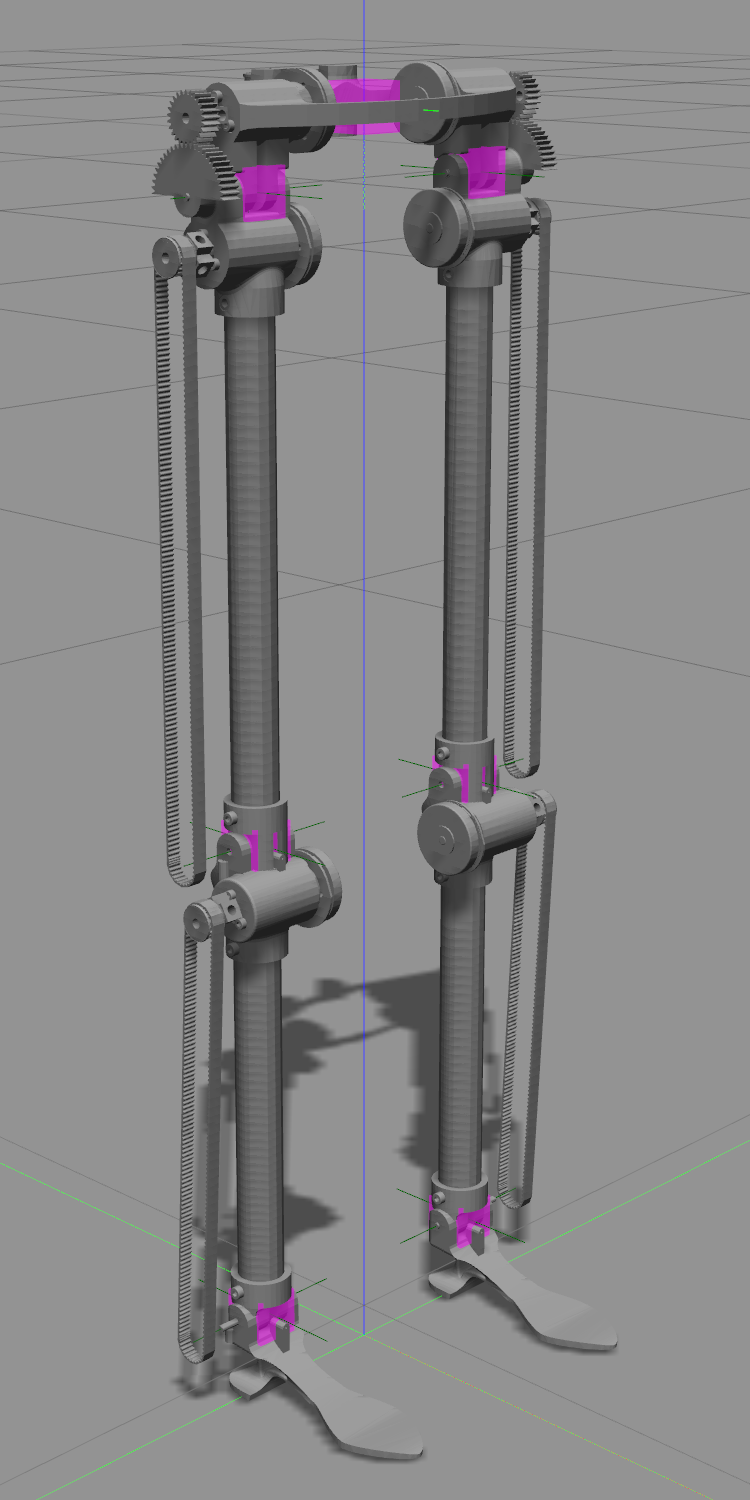
\includegraphics[width=.5\linewidth]{figures/gazebo_intertia_moments.png}
    \caption{Gazebo showing the visual model and the moments of inertia}
    \label{fig:moments_of_inertia}
  \end{subfigure}
\end{figure}

It is important to notice that the visual models and moments of inertia have been exported from the correct coordinate system.
In the case of the ankle, for example, the STL file and the moments of inertia are calculated from the coordinate system positioned in the middle of the rotational axis of the ankle, pointing the Z axis to the rotational axis and Y to the biggest extension of the part.
This can be seen in the figure \ref{fig:solidworks_ankle_coodinate_system}.

\begin{figure}[ht!]
  \centering
  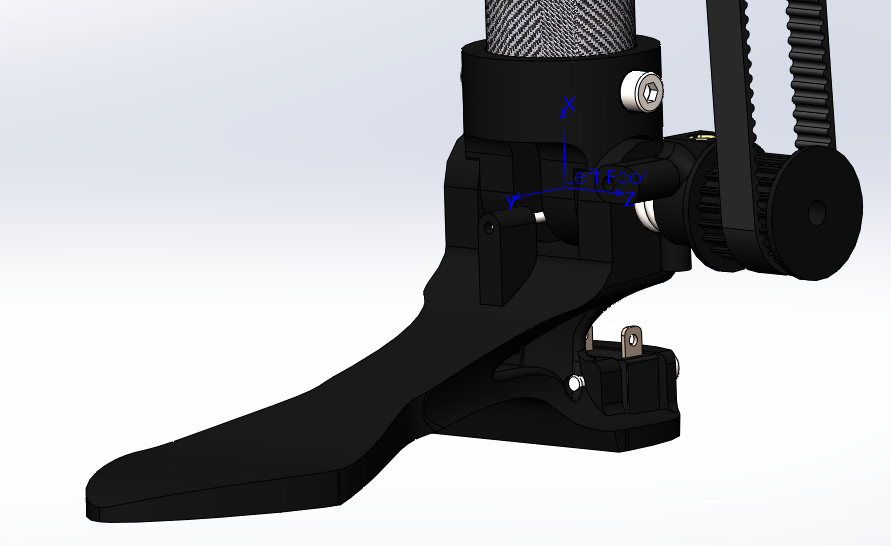
\includegraphics[width=0.75\linewidth]{figures/solidworks_ankle_coordinate_system}
  \caption{Coordinate system of the left ankle in SolidWorks}
  \label{fig:solidworks_ankle_coodinate_system}
\end{figure}

Finally, in the Xacro file the information that lacks the URDF must be added in order to simulate with Gazebo.
Eventually, to the RuBi description is added:
\begin{enumerate}
  \item \textbf{Plug-in for ROS Control}: Offers an interface for using ROS Control inside Gazebo.
  \item \textbf{Contact sensors}: Simulates contact sensors as in the feet of the real robot.
  \item \textbf{Defines friction of the components}: as the friction between the feet and the floor.
\end{enumerate}

% section robot_creation (end)
%!TEX root = ../../../report.tex
\section{Dimensional analysis} % (fold)
\label{sec:dimensional_analysis}
A problem came up when creating the robot. 
Some of the inertia moments obtained from SolidWorks, were in the order of magnitude of $10^{-8}$.
Such small number is not handled by the physics engine correctly causing the robot model to be unstable under normal conditions.

Three approaches were taken:
\begin{enumerate}
  \item \textbf{Change the physics engine}: As commented in the simulation comparison \ref{fig:simulation_comparison}, Gazebo supports multiple physics engines. Dart \cite{dart}, Simbody \cite{simbody}, Bullet \cite{bullet} and ODE \cite{ode}, where tested giving the same unstable behavior. 
  Thus, this method was discarded.
  \item \textbf{Fake the moments of inertia}: This would be to make 0 the really small moments of inertia and only leave the ones over a threshold.
  As the simulation is a qualitative analysis and no quantitative, an exact match of the moments of inertia is not needed. 
  \item \textbf{Dimensional analysis}: Based on \cite{dimensional_analysis}, the size of the robot can be increased in a proportion that make the figures big enough to be handled.
\end{enumerate}

Dimensional analysis can be applied to correlate the physical properties of the original robot with its scaled replica.
This is, if the original robot with mass $m$, volume $V$ and moment of inertia about an axis $I$, given a scale factor $s$, calculate the scaled replica $m'$, $V'$, $I'$ depending exclusively on $s$.

In the equation \ref{eq:general_inertia}, the generalized expression of the moment of inertia about an axis is shown.
\begin{equation}
\label{eq:general_inertia}
  I = \iiint_V \rho(u,v,w) |r^{2}| \,dx\,dy\,dz
\end{equation}

If the equation \ref{eq:general_inertia} is taken as the moment of inertia from the first link, the scaled one would be the shown in the equation \ref{eq:general_inertia_2}:
\begin{equation}
\label{eq:general_inertia_2}
  I' = \iiint_{V'} \rho(u,v,w)' |r^{'2}| \,dx'\,dy'\,dz'
\end{equation}

Supposing a scale factor of $s$ and as stated in the equations from \ref{eq:dx} to \ref{eq:dz}:

\begin{multicols}{3}
  \begin{equation}
  \label{eq:dx}
    \,dx=s \,dx'
  \end{equation}\break
  \begin{equation}
  \label{eq:dy}
    \,dy=s \,dy'
  \end{equation}\break
  \begin{equation}
  \label{eq:dz}
    \,dz=s \,dz'
  \end{equation}\break
\end{multicols}

Then can be deduced that $r$ increases proportionally with $s$ as shown in the Figure \ref{fig:dimensional_analysis} and presented in the equation \ref{eq:dr}:
\begin{equation}
  \label{eq:dr}
  \,r=s \,r'
\end{equation}

\begin{figure}[ht!]
  \centering
  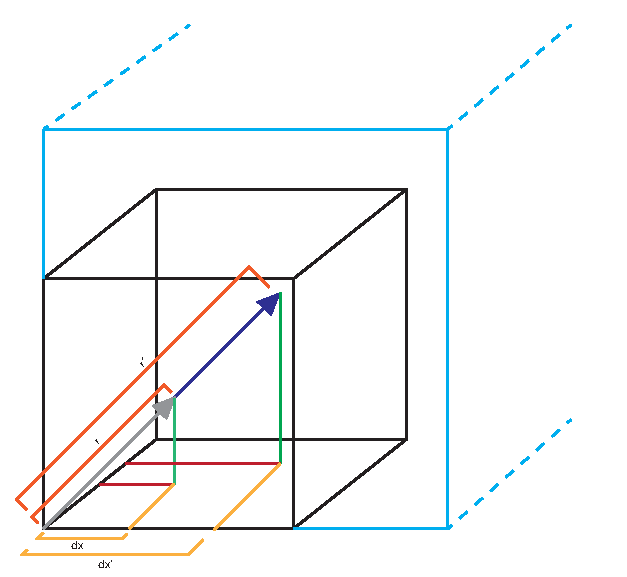
\includegraphics[width=0.5\linewidth]{figures/dimensional_analysis.pdf}
  \caption{Representation of a minimal volumentric cube.}
  \label{fig:dimensional_analysis}
\end{figure}

Assuming a constant density across all the scaled bodies, and particularizing for the moment of inertia of the center of gravity the moment of inertia is given then by \ref{eq:general_inertia_3}:
\begin{equation}
  \label{eq:general_inertia_3}
  I'_{CG} = \iiint_{V'} \rho(u,v,w)' |r^{'2}| \,dx'\,dy'\,dz' = s^{3} r_{CG}^{'2} m
\end{equation}

A correlation can be obtained for the inertia then as shown in \ref{eq:inertia_scale}:

\begin{equation}
\label{eq:inertia_scale}
  I' = \frac{s^{3} r_{CG}^{'2} m}{r_{CG}^{2} m} I = s^{5} I
\end{equation}

And lately the mass can be correlated as in \ref{eq:mass_scale}:
\begin{equation}
\label{eq:mass_scale}
  m' = V' \frac{m}{V} = s^{3}m
\end{equation}

As explained in the \ref{sec:robot_definition}, by using the Xacro format, mathematical expressions can be used.
The definition of the robot includes a set of variables in which is included $scale$ that is used to calculate $mass\_scaled$ and $inertia\_scaled$ that will modify the values of all the links to make a coherence scalable robot definition.

% section dimensional_analysis (end)
%!TEX root = ../../../report.tex
\section{Environment creation} % (fold)
\label{sec:environment_creation}
Besides the robot, other elements can be added to the simulated world.
From the Gazebo database, other robot models or parts (as a beer or a brick) can be inserted and used for any kind of experiments.

\begin{figure}[hb!]
  \centering
  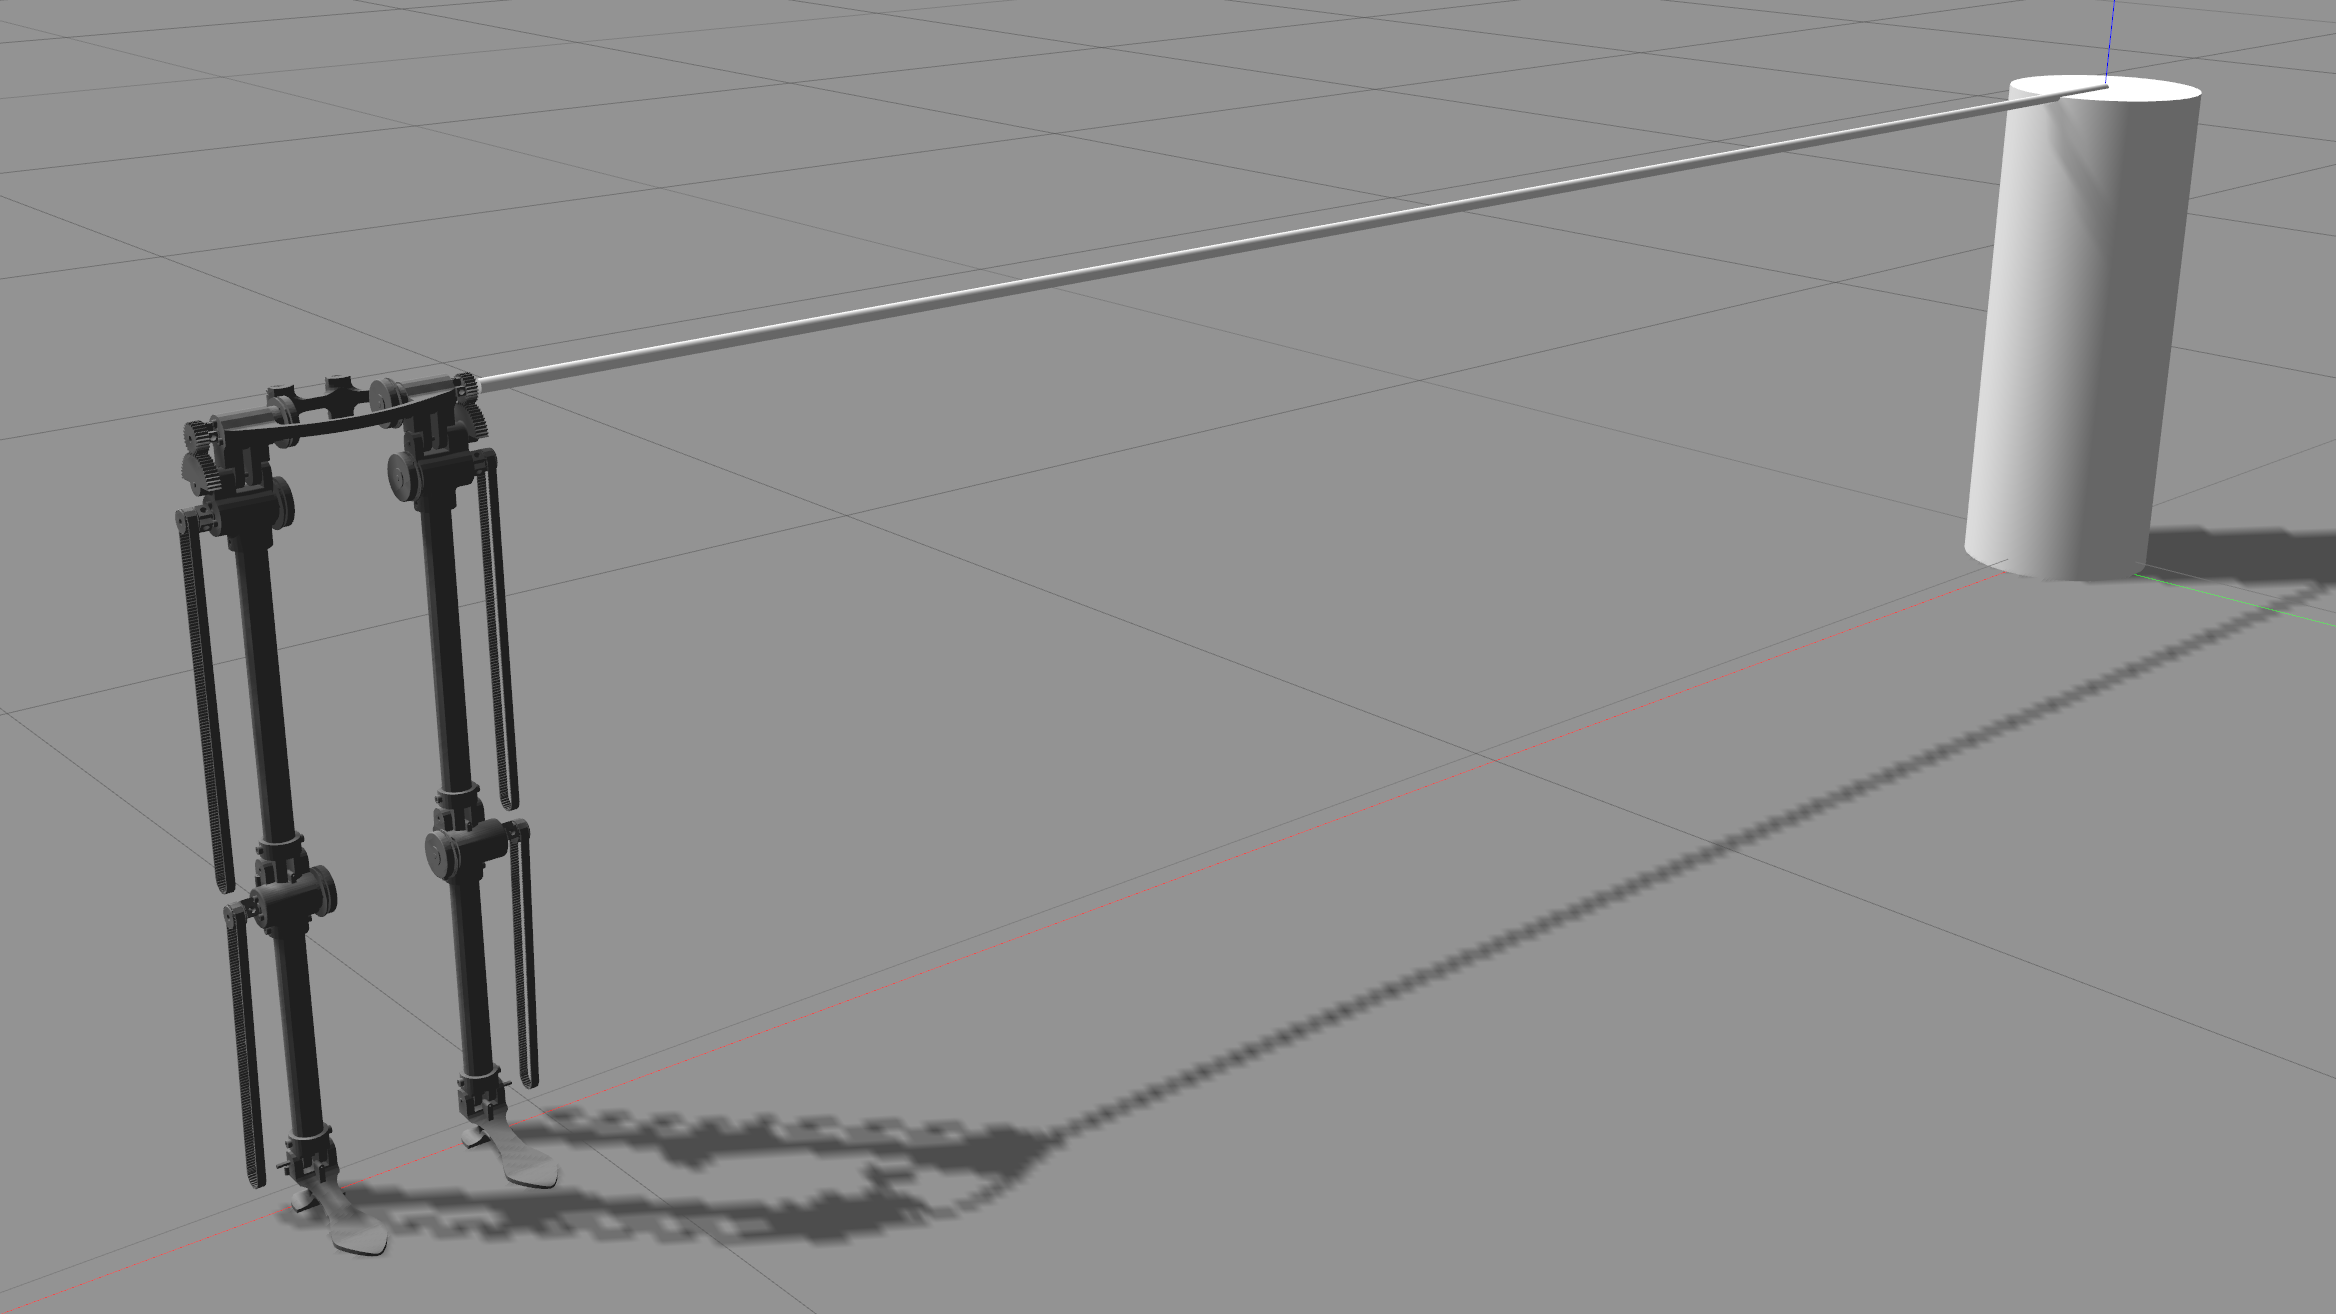
\includegraphics[width=0.75\linewidth]{figures/gazebo_rotational_holder}
  \caption{Rotational robot holder and robot}
  \label{fig:rotational_robot_holder}
\end{figure}

\hfill

In the final framework an extra tool is provided: a rotational robot holder.
It is inspired in the DACbot simulation environment in LPZ Robots, being fully parametric and reducing the degrees of freedom of the robot to constraint its motion to the scenario under study.
It can be seen in Figure \ref{fig:rotational_robot_holder}.

% section environment_creation (end)
%!TEX root = ../../../report.tex
\section{How to simulate} % (fold)
\label{sec:how_to_simulate}
The actions for starting the simulation are minimal and, with everything installed, just a terminal shall be opened and the user have to insert:

\begin{lstlisting}
roslaunch legs_gazebo legs_world.launch
\end{lstlisting}

The launch file will load ROS Control along with the simulation.
From that moment the user can run the controllers and the legs will move equally than in the real robot.
% section how_to_simulate (end)

% chapter simulation (end)

    \printbibliography
\end{document}          
